\documentclass{article}
\usepackage[utf8]{inputenc}
\usepackage{amsmath}
\usepackage{graphicx}
\usepackage[table,xcdraw]{xcolor}
\usepackage{hyperref}
\usepackage{svg}


\begin{document}
\section*{Computing transcription factor scores using TEPIC}
\subsection*{Motivation}
The main advantage of considering epigenetics data for the task of TF binding prediction is that the number of false positive predictions can be reduced \cite{pmid21106904}.
One way of incorporating epigenetics data is to reduce the genomic search space to a few candidate regions of TF binding. 
As shown before, genome-wide candidate sites for TF binding can be determined by open-chromatin experiments \cite{pmid25294828,pmid25086003,pmid22072382,pmid23424114}, e.g. peaks or footprints in DNase1-seq data, 
and/or by considering Histone marks \cite{pmid25489339,pmid25086003}, e.g. H3K4me3. 

Here, we compute TF affinities for a species specific set of \textit{Position Specific Energy Matrices (PSEM)} using \textit{TRAP} \cite{pmid17098775} which is based on a biophysical model of TF binding \cite{von1986specificity}. 
A major advantage of affinity based predictions compared to hit-based methods like Fimo \cite{Grant16022011} is that 
low-affinity binding sites can be included \cite{pmid27899623,pmid17098775}. Using the \textit{TEPIC} method, we compute TF gene scores by aggregating TF predictions calculated for a user defined set of candidate regions.
The scores, either per peak/region or gene, can be interpreted as a quantitative measurement of TF binding. 

\subsection*{Preprocessing of Position Count Matrices (PCM)}
We obtained \textit{Position Count Matrices (PCMs)} from JASPAR \cite{pmid26531826}, which is also including data from Uniprobe \cite{pmid25378322}, HOCOMOCO \cite{pmid23175603}, the Kellis Lab ENCODE Motif database \cite{pmid24335146}, and TRANSFAC \cite{pmid16381825} for five
species: \textit{homo sapiens, mus musculus, rattus norvegicus, drosophila melanogaster,} and \textit{caenorhabditis elegans}. 

Briefly, we downloaded the JASPAR CORE Vertebrata data set to cover \textit{homo sapiens, mus musculus,} and \textit{rattus norvegicus}, 
for \textit{drosophila melanogaster} we use the JASPAR CORE Insecta data set and for \textit{caenorhabditis elegans} we obtained the JASPAR CORE Nematoda PCMs.
From HOCOMOCO we use the provided data for \textit{homo sapiens} and \textit{mus musculus}. The latter is also used for \textit{rattus norvegicus}. 
The Kellis Lab ENCODE Motifs are based on human ChIP-seq data. Thus, we consider these \textit{PCMs} for \textit{homo sapiens, mus musculus}, and \textit{rattus norvegicus}.
From TRANSFAC, we obtained species specific sets for all considered organisms. 

From this initial set, we removed all TFs that could not be mapped to an Ensembl gene ID, using the Ensemble Genes 87 database, 
and the current versions of the reference genomes: GRCh38, GRCm38, Rnor\_6, BDGP6, and WBcel235. 
Thereby, we generate species specific sets of \textit{PCMs} assuming a motif conservation
among vertebrates for the JASPAR CORE Vertebrata \textit{PCMs}, the HOCOMOCO mouse \textit{PCMs}, and Kellis Lab ENCODE Motif \textit{PCMs}.
Neither HOCOMOCO nor Kellis Lab ENCODE Motifs are considered for \textit{drosophila melanogaster} and \textit{caenorhabditis elegans}.

Next, for each species set, we computed the information content $IC$ of each \textit{PCM} $M$  normalized per motif length $|M|$ as
\begin{align}
P(i,j)= \frac{M(i,j)+pc}{4*pc+\sum_{i}M(i,j)}, \\
IC=-\frac{\sum_{ij}log(P(i,j)*P(i,j)}{|M|},
\end{align}
with $i \in \{A,C,G,T\}$, $j \in \{1,...|M|\}$, and a pseudo count $pc=1$.
\bigskip
\\Note that the smaller the $IC$ value of a matrix, the more informative the matrix is.

In Figure \ref{IC-Content}, a violin plot shows the distribution of the normalized information content for the \textit{homo sapiens} data set. 
Across all species collections, we find that the JASPAR matrices have a small variance and that the poorest JASPAR \textit{PCM} 
is still more informative than several \textit{PCMs} from other databases.
Therefore, we decided to consider all JASPAR \textit{PCMs} and use the normalized information content value of the poorest JASPAR \textit{PCM} as a species specific cut-off value for the remaining databases. The cut-offs are:
\begin{itemize}
\item \textit{homo sapiens: } $1.55928$
\item \textit{mus musculus: } $1.55928$
\item \textit{rattus norvegicus: $1.55928$ }
\item \textit{drosophila melanogaster: $1.67157$}
\item \textit{caenorhabditis elegans: $1.33879$}
\end{itemize}
\begin{figure}[h!]
\begin{center}
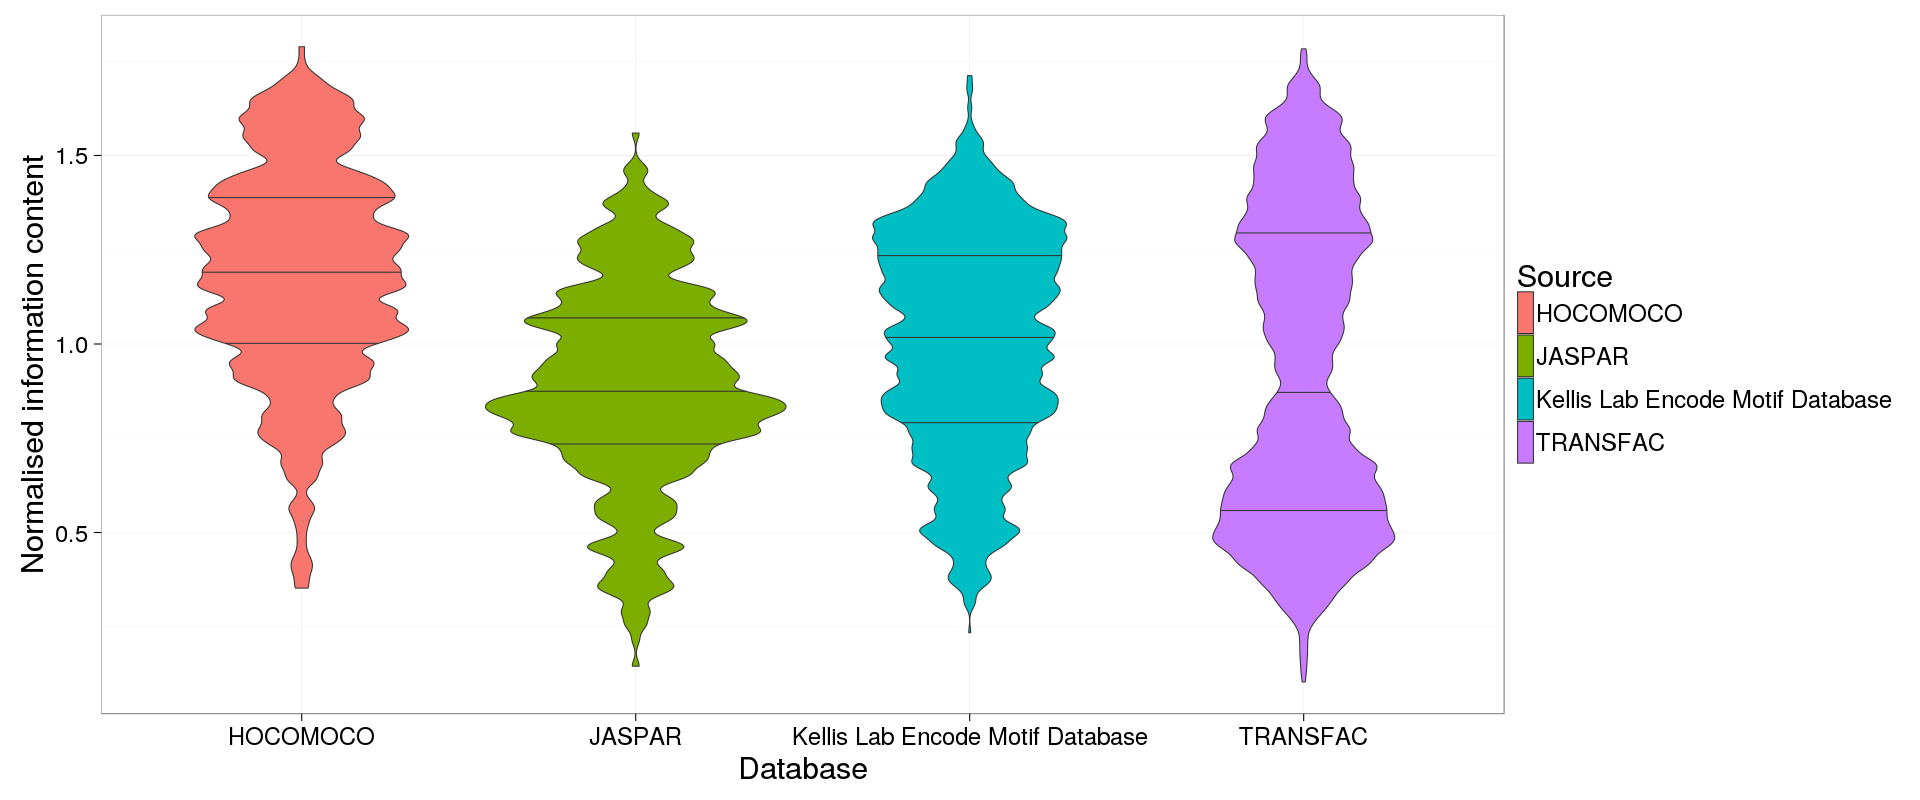
\includegraphics[width=\textwidth]{Information_Content_Violin_Plot.png}
\end{center}
\caption{Normalized information content for \textit{PCMs} extracted from JASPAR Core Vertebrata, HOCOMOCO human, the Kellis ENCODE Motif database, and TRANSFAC Human. 
Small values indicate high quality matrices. Clearly, the poorest \textit{PCM} in JASPAR is still better than several \textit{PCMs} out of the other databases.}
\label{IC-Content}
\end{figure}
In case that multiple motifs exists for one distinct TF in one database, we consider only the \textit{PCM} with the best $IC$ value. 
If the motifs are marked specifically as a secondary or tertiary binding motif, as in JASPAR, we do not remove them. 

In order to merge the different databases per species, we execute the following merging procedure on the filtered sets of the individual databases:
\begin{enumerate}
\item Consider all JASPAR matrices.
\item Add all HOCOMOCO matrices that are not included in the set of step (1).
\item Add all Kellis Lab ENCODE Motif database matrices that are not included in the set of step (2).
\item Add all TRANSFAC matrices that are not included in the set of step (3).
\end{enumerate}
This procedure ensures that we generate the largest possible set of open-source \textit{PCMs} from our collection of TF binding motifs. In addition to the unified set,
we also provide the user with the option to work with all \textit{PCMs} from a single database. 
\bigskip
\\As mentioned above, \textit{TRAP} computes TF affinities that are based on a biophysical model of TF binding.
Therefore \textit{PCMs} have to be converted to \textit{Position Specific Energy Matrices (PSEMs)} such that they can be used in \textit{TRAP}.
Intuitively, \textit{PSEMs} represent the mismatch energy of a given motif. For a detailed explanation and motivation of the energy based score, please check \cite{pmid17098775}.
A \textit{PCM M} is converted to a \textit{PSEM E} according to:
\begin{align}
E_{i,j}=\frac{1}{\lambda}log(\frac{M_{max,j}}{M_{i,j}}b_{i,j}), \\
M_{max,j}=\max\limits_{i\in\{A,C,G,T\}}(M_{i,j}).
\end{align}
The parameter $\lambda$ is used for scaling the mismatch energies and $b_{i,j}$ denotes the background frequency of the nucleotide $i$ with respect to the most frequent nucleotide at position $j$. 
This conversion formula is part of the mismatch energy postulated in formula (4) in \cite{pmid17098775}. 
By definition, if $j=max$, than $E_{i,j}=0$, as there should be no mismatch energy for the best possible sequence match. 
Note that, during conversion, a pseudo count $pc = 1$ is added to each $M_{i,j}$. 

The conversion is done by a C++ tool provided by the authors of \textit{TRAP}. This is also included in the \textit{TEPIC} repository.
As suggested in \cite{pmid17098775}, we use the following parameters for the conversion:
\begin{itemize}
\item $\lambda=0.7$
\item $m=0.584$
\item $n=-5.66$
\end{itemize}
The parameters \textit{slope m} and \textit{intercept n} are used to compute a matrix specific parameter $R_0$ that combines the concentration of the corresponding TF and the
equilibrium constant of the binding reaction with its optimal binding site as defined in \cite{pmid17098775}. The authors of \textit{TRAP} found a linear approximation for $R_0$ with:
\begin{align}
ln(R_0)=m*|M|+n,
\end{align}
where $|M|$ denotes the length of the \textit{PCM} as above.
\bigskip
\\Further, we exploit species specific GC-content values:
\begin{itemize}
\item \textit{homo sapiens }$=0.41$
\item \textit{mus musculus }$=0.42$
\item \textit{rattus norvegicus }$=0.42$
\item \textit{drosophila melanogaster }$=0.43$
\item \textit{caenorhabditis elegans }$=0.36$
\end{itemize}
Table \ref{Matrices2} shows the number of \textit{PCMs} that based the quality filtering and the within database redundancy check. 
Table \ref{Matrices} provides an overview on the final counts of the unified set of PCMs.
The entire processing workflow of \textit{PCMs} to \textit{PSEMs} is shown in Figure \ref{PCM-Workflow}.

\begin{table}[h!]
\centering
\small
\begin{tabular}{|c|c|c|c|c|}
\hline
\textit{\textbf{}} & Jaspar & Hocomoco & \multicolumn{1}{c|}{\begin{tabular}[c]{@{}c@{}}Kellis Lab Encode \\ Motif Database\end{tabular}} & Transfac \\ \hline
\begin{tabular}[c]{@{}c@{}}Homo \\ sapiens\end{tabular} & 515 & 390 & 559 & 1747 \\ \hline
\begin{tabular}[c]{@{}c@{}}Mus \\ musculus\end{tabular} & 499 & 261 & 523 & 921 \\ \hline
\begin{tabular}[c]{@{}c@{}}Rattus \\ norvegicus\end{tabular} & 489  & 253 & 513 & 389 \\ \hline
\begin{tabular}[c]{@{}c@{}}Drosophila \\ melanogaster\end{tabular} & 129 & 0 & 0 & 290  \\ \hline
\begin{tabular}[c]{@{}c@{}}Caenorhabditis \\ elegans\end{tabular} & 26 & 0 & 0 & 42  \\ \hline
\end{tabular}
\caption{Overview on \textit{PCM} counts per species and database after quality filtering and a within database redundancy check.}
\label{Matrices2}
\end{table}

\begin{table}[h!]
\centering
\small
\begin{tabular}{|c|c|c|c|c|c|}
\hline
\textit{\textbf{}} & Jaspar & Hocomoco & \multicolumn{1}{c|}{\begin{tabular}[c]{@{}c@{}}Kellis Lab Encode \\ Motif Database\end{tabular}} & Transfac & \multicolumn{1}{l|}{Total} \\ \hline
\begin{tabular}[c]{@{}c@{}}Homo \\ sapiens\end{tabular} & 515 & 81 & 130 & 584 & 1310 \\ \hline
\begin{tabular}[c]{@{}c@{}}Mus \\ musculus\end{tabular} & 499 & 67 & 124 & 194 & 884 \\ \hline
\begin{tabular}[c]{@{}c@{}}Rattus \\ norvegicus\end{tabular} & 489 & 67 & 121 & 50 & 727 \\ \hline
\begin{tabular}[c]{@{}c@{}}Drosophila \\ melanogaster\end{tabular} & 129 & 0 & 0 & 92 & 221 \\ \hline
\begin{tabular}[c]{@{}c@{}}Caenorhabditis \\ elegans\end{tabular} & 26 & 0 & 0 & 14 & 40 \\ \hline
\end{tabular}
\caption{Overview on \textit{PCM} counts per species and database after quality and redundancy filtering. We considered all Jaspar matrices and added additional non redundant \textit{PCMs} from Hocomoco, the Kellis Lab Encode Motif Database, and Transfac.}
\label{Matrices}
\end{table}

\begin{figure}[h!]
\begin{center}
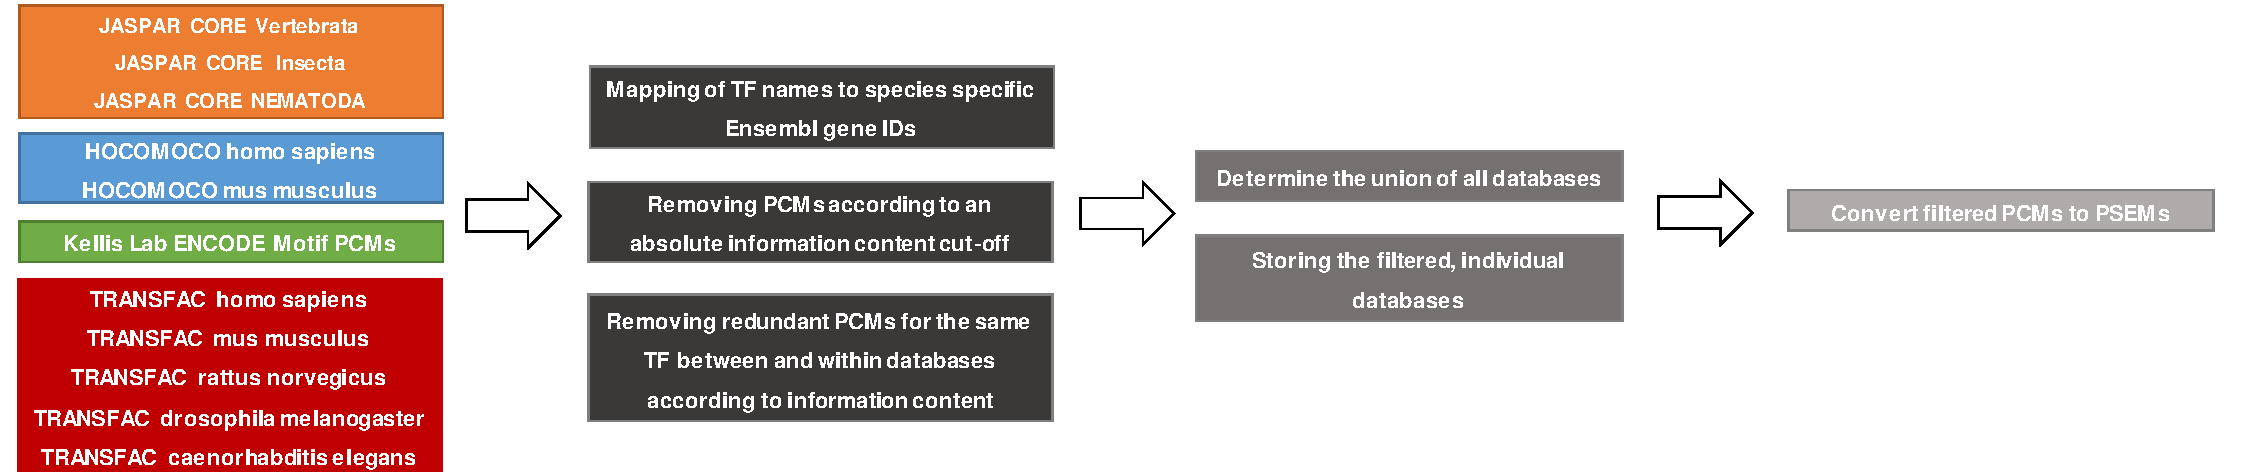
\includegraphics[width=\textwidth]{PCM_Processing_RegulatorTrail.pdf}
\end{center}
\caption{Visualization of the PCM preprocessing workflow.}
\label{PCM-Workflow}
\end{figure}

\newpage
\mbox{}
\newpage
\subsection*{Computing TF gene scores}
Currently, we offer the annotation of five different species, including the most common model organisms: 
\textit{homo sapiens, mus musculus, rattus norvegicus, drosophila melanogaster,} and \textit{caenorhabditis elegans}.
Using our collections of species specific \textit{PSEMs}, \textit{TRAP} computes TF binding affinities in all user provided regions 
that could be found in the reference genomes of the respective species and 
overlap with a window of user defined size $w$ that is centered at the most $5'$ TSS of all annotated genes in the considered organism. 
Then, TF gene scores are computed by incorporating all candidate binding sites within the window centered around the $5'$ TSS of genes in the final score. 
The contribution of the individual sites is weighted by their distance to the selected TSS with an exponential decay function \cite{pmid19995984}.
Formally, the TF gene score $a_{g,i}$ for gene $g$ and TF $i$ is computed as
\begin{align}
a_{g,i}^{w}&=\sum_{p \in P_{g,w}} a_{p,i}e^{-\frac{d_{p,g}}{d_0}},
\end{align}
where $a_{p,i}$ is the affinity of TF $i$ in peak $p$, the set $P_{g,x}$ contains all open-chromatin peaks
in a window of size $w$ around gene $g$, $d_{p,g}$ is the distance from the center of peak $p$ to the TSS of gene $g$, and $d_0$ is a constant fixed at $5000$bp \cite{pmid19995984}.
Additionally, affinities can be normalised by peak(and motif)-length during the computation of gene-TF scores:
\begin{align}
a_{g,i}^{w}&=\sum_{p \in P_{g,w}} {\frac{a_{p,i}}{|p|-|m|}e^{-\frac{d_{p,g}}{d_0}}},
\end{align}
where $|p|$ is the length of peak $p$, $|m_i|$ is
the length of the motif of TF $i$, with a extra count of $1$.
If the signal within a peak should be directly considered in the gene-TF score, we compute:
\begin{align}
a_{g,i}^{w}&=\sum_{p \in P_{g,w}} {\frac{a_{p,i}}{|p|-|m|}s_{p}e^{-\frac{d_{p,g}}{d_0}}},
\end{align}
where $s_p$ is the per base signal in peak $p$. This computation can be done with and without length normalisation of the affinities. 
The workflow of TEPIC is depicted in Figure \ref{workflowFig}.

In addition to the TF gene scores, TEPIC can compute features for peak length, peak count, and peak signal following the same scoring formulation as for
TF affinities. These features can be used for example to assess the influence of chromatin accessiblity on gene expression without considering TF binding
predictions. 
\begin{figure}[h!]
\begin{center}
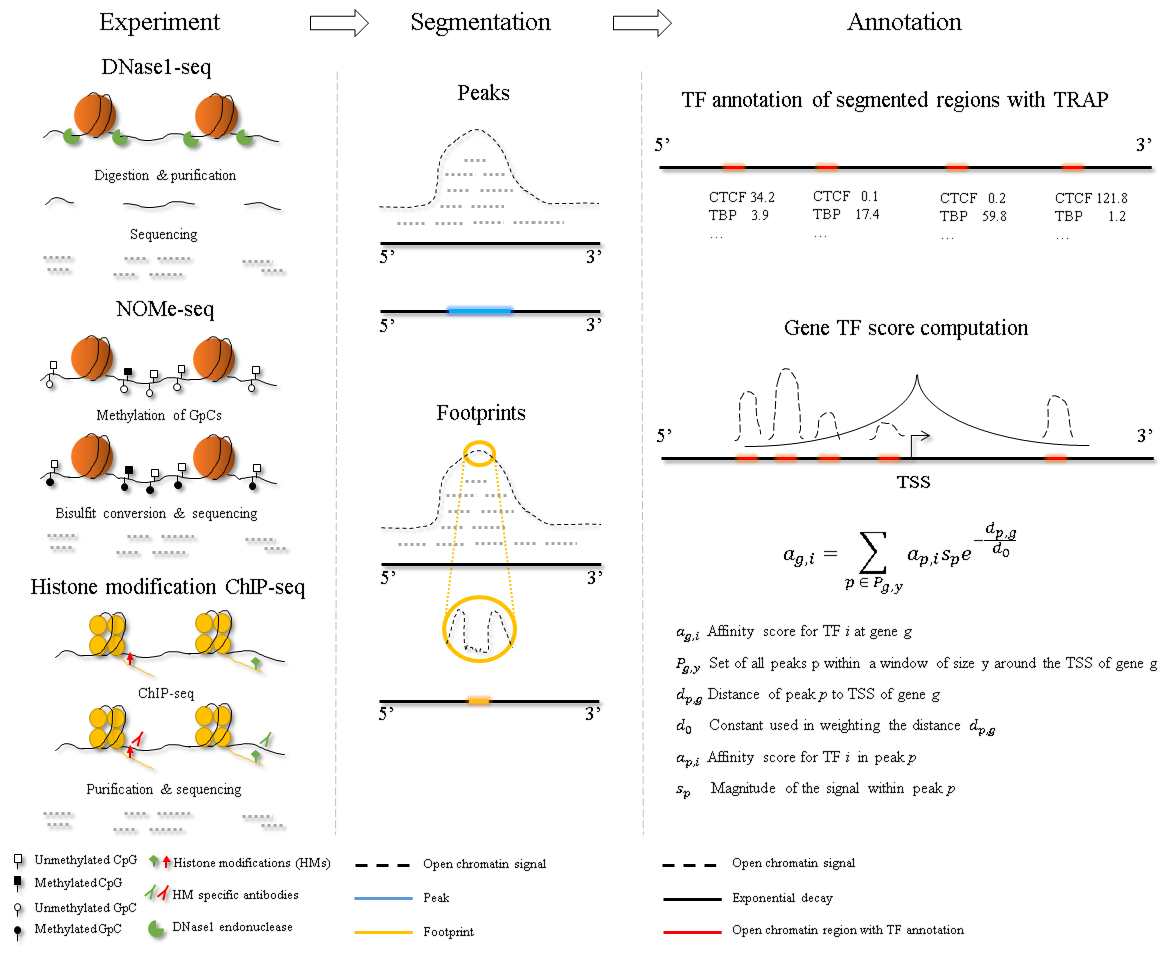
\includegraphics[width=\textwidth]{Workflow.png}
\end{center}
\caption{The general workflow of \textit{TEPIC} is as follows: 
Data of an open-chromatin or Histone modification ChIP-seq experiment needs to be preprocessed to generate a genome segmentation, 
either by peak for footprint calling. 
Using the segmentation, \textit{TEPIC} applies \textit{TRAP} in all regions of interest, and computes TF gene scores using exponential decay to reweigh 
TF binding predictions in open-chromatin regions based on their distance to a genes TSS.} 
\label{workflowFig}
\end{figure}

\newpage
\subsection*{Required input}
To compute TF gene scores a user needs to specify:
\begin{itemize}
\item a reference genome,
\item a set of \textit{PSEMs},
\item a set of genomic regions in BED format.
\end{itemize}
Note that the chromosome identifiers in the BED file must match the identifiers used in the reference genomes, neglecting the \textit{chr} prefix. 
Otherwise they can not be considered. 
Special care should be taken for \textit{caenorhabditis elegans}, as Roman digits are used for enumeration of chromosomes.

\subsection*{Output}
This step generates the following output:
\begin{enumerate}
\item TF affinities for all selected \textit{PSEMs} in the regions provided by the user that passed the filtering step. 
\item (Length normalised) TF gene scores for all selected \textit{PSEMs} calculated as described above (optionally including peak features). 
\item A meta data file listing all used parameters.
\item Optionally a seperate file containing the signal information in peaks. 
\end{enumerate}

\newpage

\section*{Identification of key transcriptional regulators using epigenetics data (INVOKE)}
Epigenetics data contains a wealth of information on gene regulation. It was shown that especially
data on open-chromatin is well suited to build predictive models of gene-expression \cite{pmid27899623,pmid22955983,pmid25231769,pmid22954627}.
Interpreting these models allows the inference of regulators that may play a key role in gene-expression regulation.
\bigskip
\\Hear, we offer an integrated analysis of epigenetics data, e.g. open-chromatin data (DNase1-seq, ATAC-seq, NOMe-seq) and gene-expression data
to suggest key transcriptional regulators in the analysed sample.
\bigskip
\\Note that, although incorporating epigenetic data greatly improved the performance of TF binding predictions, both computing TF binding predictions and linking TFs to genes are still unsolved problems and all predictions
should be seen as suggestions and not as the absolute truth.
\bigskip
\\The \textit{INVOKE} analysis is split up into two main steps. 
\begin{enumerate}
\item Computing TF gene scores on the basis of epigenetic data using \textit{TEPIC} (see above).
\item Learning a linear regression model to predict gene expression from TF gene scores computed in (1).
\end{enumerate}

\subsection*{Linear regression to predict gene expression}
\subsubsection*{Motivation}
In order to learn about potentially important regulators, we build a linear, interpretable regression model, 
comparable to methods proposed in \cite{pmid27899623,pmid22955983,pmid25231769,pmid22954627}.
Here, we use TF gene scores computed with \textit{TEPIC} as features in a linear regression setup to predict gene expression.
In such a \textit{per sample} approach, we stick to the simplifying assumption that all genes are regulated similarly. 
Features with a high regression coefficient can be suggested to be key regulators in the analysed sample, as they seem to effect the expression
of a large portion of the genes under consideration. However, the results of this method should be seen as suggestions for possible regulators and not as the absolute truth. 

Details on the learning setup and on the available regularization methods are provided in the next section.

\subsubsection*{Available regularization methods}
We offer three different regularization techniques:
\begin{itemize}
\item Lasso:
\begin{align}
 \hat{\beta}&=\underset{\beta}{\arg\,min} ||y-X\beta||^2 + ||\beta||,
\end{align}
\item Ridge:
\begin{align}
 \hat{\beta}&=\underset{\beta}{\arg\,min} ||y-X\beta||^2 + ||\beta||^2,
\end{align}
\item Elastic net:
\begin{align}
 \hat{\beta}&=\underset{\beta}{\arg\,min} ||y-X\beta||^2 + \alpha||\beta||^2 + (1-\alpha)||\beta||,
\end{align}
\end{itemize}
where, $\beta$ represents the regression coefficient vector, $\hat{\beta}$ represents the estimated coefficients, $X$ is the feature matrix, $y$ is the response vector, and
the parameter $\alpha$ controls the distribution between Ridge and Lasso penalty in the elastic net.
\bigskip
\\Using Lasso regularization, models are sparse and can be learned very fast. 
But, Lasso can not properly deal with correlated features, e.g. instead of distributing the coefficients among them, only one is selected. Also, Lasso solutions are not stable and therefore should be interpreted with caution. Nevertheless, Lasso regularization is good to get a first impression of model performance. 

The disadvantage of Ridge regression is that it can not produce sparse models (many coefficients being exactly 0), which may hinder interpretability. 

Elastic net regularization was designed to overcome the limitations of both regularization techniques mentioned above.
It resolves the correlation between features by distributing the feature weights among them, and simultaneously leads to sparse and stable models \cite{Zou05regularizationand}. 
However, learning a model using elastic net penalty is slower than using either only Lasso or Ridge regularization.

\subsubsection*{Details on the learning setup}
The data matrix $X$, containing TF gene scores, and the response vector $y$, containing gene expression values, are log-transformed, 
with a pseudo-count of $1$, centered and scaled to fit them as. 
Regression coefficients are computed in a inner cross validation,
the $\alpha$ parameter of elastic net regularization is optimized with a default step size of $0.1$.

We offer two ways to use our learning pipeline:
\begin{enumerate}
\item{Learn a model for feature interpretation without computing performance measures:
In order to provide a time efficient way of obtaining an interpretable model and to prevent a potential loss of information
by considering only a portion of the full data set for model training, the regression coefficients are determined on the entire data set.}
\item{Learn a model for feature interpretation and compute model performance: 
Nested cross-validation is used to learn the models and to assess their performance. 
Per default, $20\%$ of the data are used as test data and $80\%$ are used as training data. 
Model performance is assessed in an outer cross validation. 
We report the mean pearson correlation, the mean spearman correlation, and the mean squared error over the outer folds as measures of model performance.
Additionally, a model is learned on the entire data set as described in (1) for interpretation of the coefficients.}
\end{enumerate}
All parameters mentioned in this section can be changed by the user. The learning process is sketched in Figure \ref{learningFig}.

\subsubsection*{Required input}
In addition to the input required for the computation of TF gene scores in TEPIC, a file containing gene expression data must be provided.
This file should be structured such that column $1$ contains the gene identifiers and column $2$ holds expression values.
Besides, we support the upload of a matrix containing gene expression data for several samples. In that case, the user has to select the column/sample that should
be used for model construction. 

\subsubsection*{Output and hints for interpretation}
The user is always provided with the following files:
\begin{itemize}
\item a list of regression coefficients computed on the entire data set,
\item a bar plot showing the regression coefficients with an absolute value $> 0.025$.
\end{itemize}
The larger a regression coefficient, the stronger is the inferred effect of the corresponding TF on gene expression. Positive coefficients suggest an activating influence of TFs,
negative coefficients suggest an inhibiting effect. 

If model performance was assessed, the following is available in addition:
\begin{itemize}
\item a summary on model performance containing the aforementioned measures (pearson correlation, spearman correlation, mean squared error),
\item a list of regression coefficients determined in the outer cross validation,
\item a heatmap visualizing the regression coefficients determined in the outer cross validation for at most the top $10$ positive and negative features, sorted according to their mean.
\item an image showing a box plot for pearson and spearman correlation respectively.
\item scatter plots showing the predicted vs the measured gene expression for each outer cross validation fold.
\end{itemize}
The heatmap can be easily used to judge model performance, as it shows the regression coefficients of all outer-cross validation runs. The box plots provide further insights into model performance and stability across the outer folds of the cross validation.
\vspace{1cm}
\begin{figure}[h!]
\begin{center}
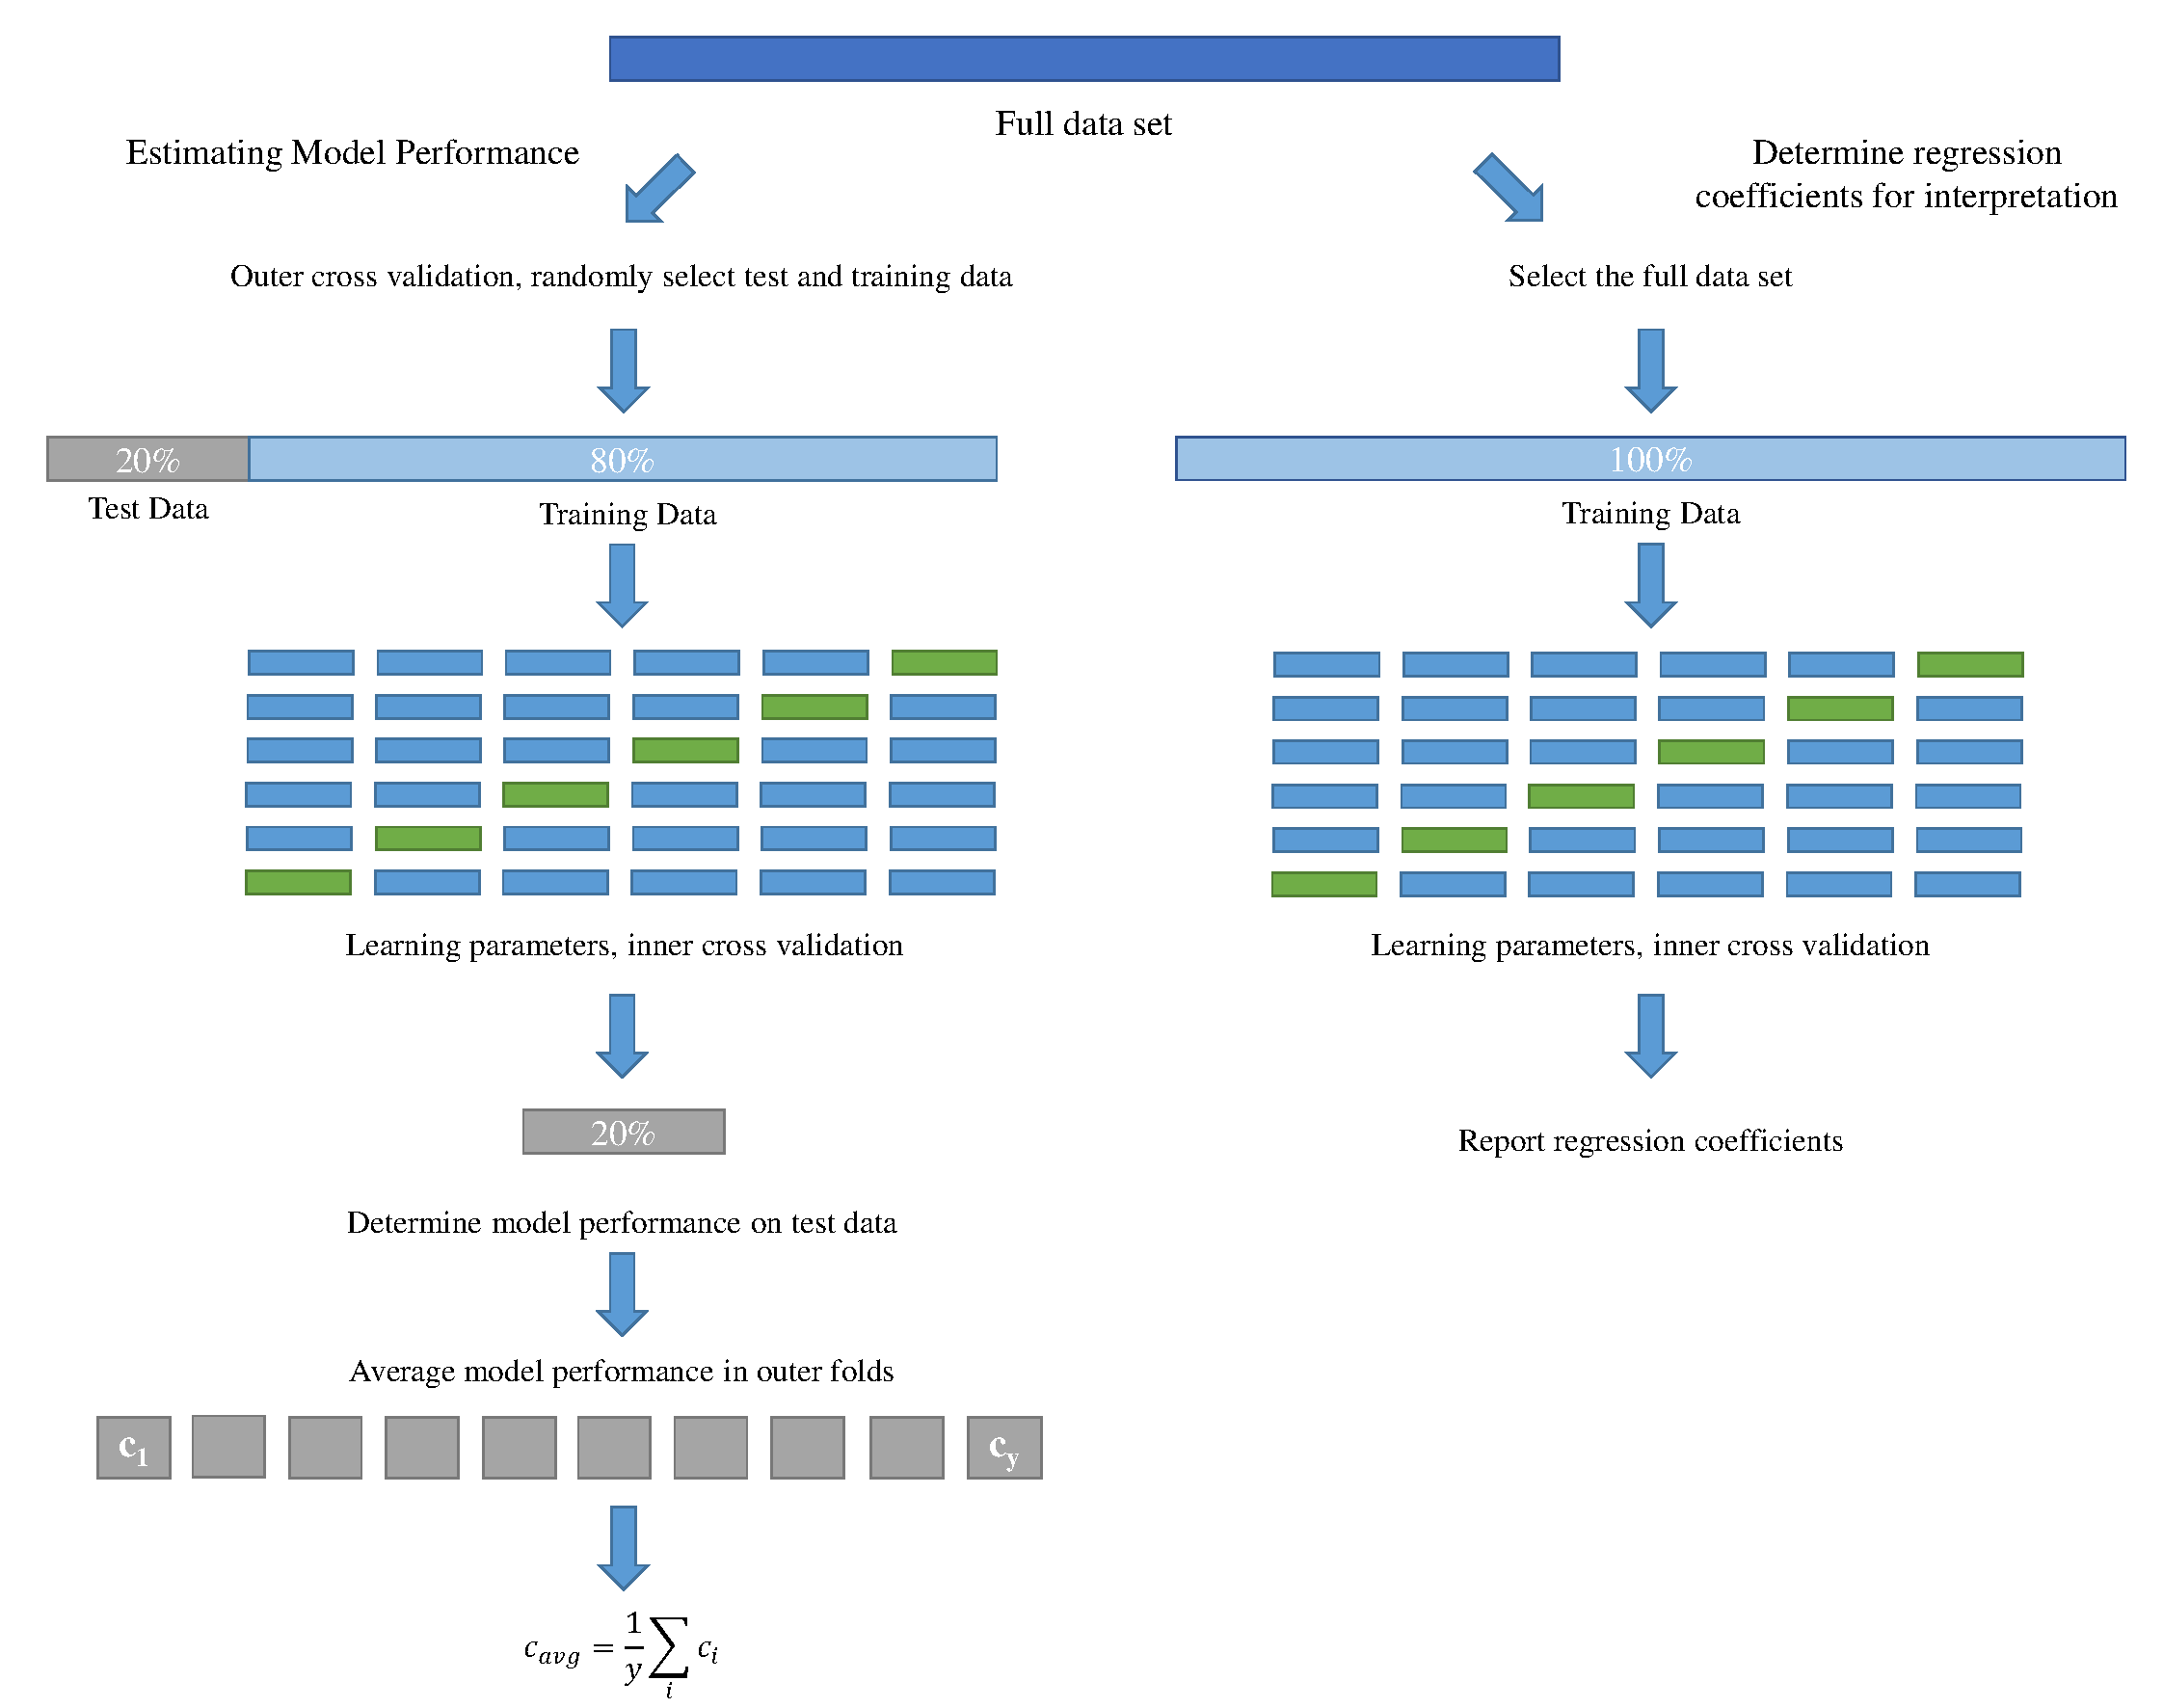
\includegraphics[width=\textwidth]{Learning.pdf}
\end{center}
\caption{Overview of the learning process. 
The left part of the Figure describes the assessment of model performance in a $y$-fold outer cross validation and $6$-fold inner cross validation. 
The right hand site illustrates model training on the entire data set, again using a $6$-fold inner cross validation for parameter learning.}
\label{learningFig}
\end{figure}

\newpage
\mbox{}
\newpage
\section*{Differential analysis to identify novel transcriptional regulators for differentially expressed genes (DYNAMITE)}
Although a variety of methods have been proposed to generate genome-wide TF binding predictions [\cite{pmid27899623,pmid22072382,pmid23424114,pmid25086003}] and to establish \textit{TF to tissue} 
associations [\cite{pmid22955983,pmid19995984,pmid27899623}], systematic, feasible, and easy to use ways of linking TFs to distinct genes are rare. 

In addition to the \textit{INVOKE} analysis, we propose a method to infer the most likely transcriptional regulators for a set of differentially expressed genes. 
We use TF scores, computed using \textit{TEPIC}, and logistic regression to identify TFs that have explanatory power to distinguish between up- and down-regulated genes. 

\section*{Input}
To run \textit{DYNAMITE}, a user most provide candidate regions of TF binding for two groups of samples, $A$ and $B$, e.g. control and disease. 
These can be derived, for example, by open chromatin experiments such as DNase-seq. 
It is essential that the candidate regions reflect the characteristics of chromatin organization in the analysed tissues. 
In addition, a list of differential expressed genes between two groups as well as log2 fold changes of the expression are needed. 

\section*{Method}
Our method consits of two parts: (1) gene-TF score computation, and (2) identification of key TFs. 
\subsection*{Step 1: Computing Gene-TF Scores}
Using TEPIC, we compute gene-TF scores $g_{ij}$ for all differentially expressed genes $i$ and distinct TFs $j$ considering the provided candidate regions for all replicates $a$ of group $A$ and for all replicates $b$ of group $B$. 
As a result, gene-TF matrices $M_k$ for all replicates of both groups are obtained. To account for biological variation among the replicates, we compute two matrices $M_A$, $M_B$ holding the the mean gene-TF scores among all replicates of a group, where
\begin{align}
 M_{A_{ij}}= \frac{\sum_{a \in A}{M_{a_{ij}}}}{|A|},
 \\M_{B_{ij}}= \frac{\sum_{b \in B}{M_{b_{ij}}}}{|B|}.
\end{align}
Using matrices $M_A$ and $M_B$ we compute a matrix $R_{AB}$ that holds the ratios of gene-TF scores for all genes and all TFs:
\begin{equation}
    R_{AB_{ij}}=\frac{M_{A_{ij}}}{M_{B_{ij}}}.
\end{equation}
Thus, $R_{AB}$ represents the changes in TF binding between groups $A$ and $B$ on a gene level.
The feature computation is sketched in Figure \ref{TF-Gene-Score_Computation}.
\begin{figure}[h!]
\centering
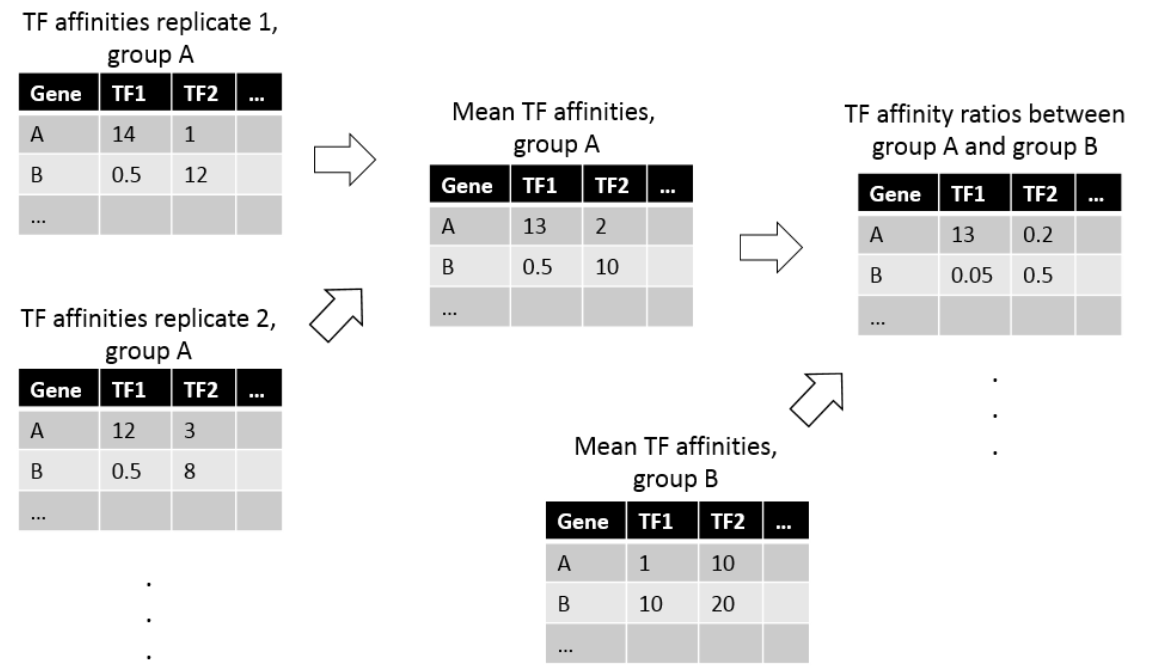
\includegraphics[width=0.75\textwidth]{TF_Affinities.png}
\caption{Computation of differential TF features between two groups.}
\label{TF-Gene-Score_Computation}
\end{figure}
\subsection*{Step 2: Identification of Key Transcription Factors}
To identify those TFs that can explain the differential expression state of as many genes as possible, we build a logistic regression classifier. 
We use matrix $R_{AB}$ computed in Step $1$ as the feature matrix $X$, and a binary vector of gene expression changes as response $y$. 
An example is shown in Figure \ref{Log-Reg-Example}.
\begin{figure}[h!]
\centering
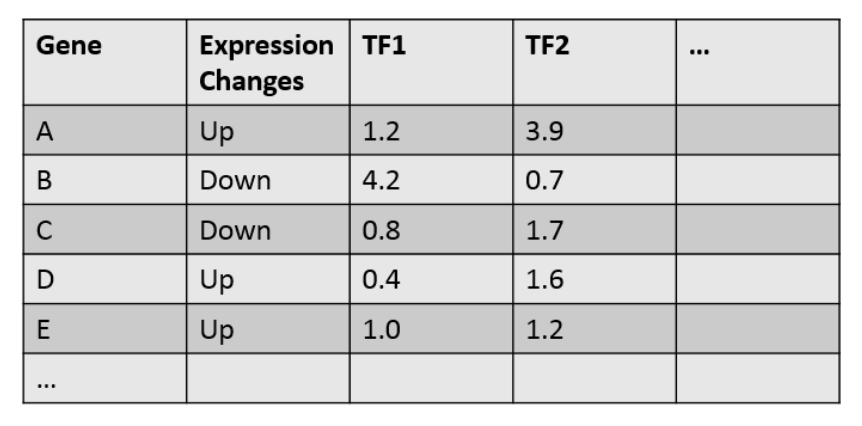
\includegraphics[width=0.5\textwidth]{Example_Matrix.png}
\caption{Example for an matrix used as input to the logistic regression. The column \textit{Expression Changes} is used as response, while the affinity ratios \textit{TFx} are used as features.}
\label{Log-Reg-Example}
\end{figure}
We perform logistic regression with elastic net regularisation (11).
As above, we tune the parameter $\alpha$ that distributes the weight between lasso and ridge penalty in a grid search with user defined step-size between $0$ and $1$.

Model parameters are learned in an inner cross validation, while the accuracy of our classifier can be assessed through an outer cross validation. This is the
same learning paradigm that is described for the \textit{INVOKE} analysis (Figure \ref{learningFig}). We use the entire dataset for model training and to interpret the regression coefficients.
TFs that correspond to features with a non-zero regression coefficient can be seen as being essential to explain the observed expression differences and should be further investigated.

\section*{Output}
Model performance is reported in a \textit{txt} file and visually in a bar plot using mean test and training accuracy as well as the F1 measure.
A heatmap shows the regression coefficients in the outer cross validation folds. 
Additionaly, we report confusion matrices for the outer cross validation folds.
We generate a bar-plot with the regression coefficients of all TFs selected in the final model.
A positive coeffcient is used by the model to predict genes as upregulated, a negative coefficient is related to genes that are predicted as downregulated. The interpretation
of the model can be simplified if the user makes sure that both TF ratios and gene expression fold changes are computed in the same order. 

We provide an additional script to generate further plots per feature that can help to understand the model. As shown in Figure \ref{ExampleAnalysisOfDynamite},
density plots, and scatter plots are generated to help elucidating why a particular feature was selected by the model.
\begin{figure}[h!]
\centering
\includesvg[width=\textwidth]{Feature_overview_TEMvsTN_Peak_Counts}
\caption{Example for a automatically created feature analysis Figure generated on the example data provided in the repository. The density plots show the distribution of TF affinities, the
scatter plot relat the TF affinities to the observed expression changes. The miniature heatmap shows the regression coefficients determined during the outer cross validation.}
\label{ExampleAnalysisOfDynamite}
\end{figure}

\newpage
\mbox{}
\newpage

\subsection*{Determine important transcriptional regulators from time serires data (EPIC-DREM)}
\textit{EPIC-DREM} is a combination of \textit{TEPIC}  and the \textit{Dynamic Regulatory Events Miner (DREM)} \cite{pmid17224918}.
Instead of using static ChIP-seq data, which is provided in \textit{DREM 2.0}, we suggest to use time-point specific TF binding predictions
based on time-dependent epigenomic profiles. Thereby, \textit{DREM} can infer regulators that can be linked to expression changes at distinct points in time.
We have shown that using the predicted, dynamic TF binding events is superior to the static data included in \textit{DREM}.

In order generate a sparse input matrix for \textit{DREM}, we devised a strategy to threshold TF affinities based on a set of background sequences.
These can be either chosen automatically or be provided by the user. Please check the README file for detailed options. 

In Figure \ref{epicdrem}, we illustrate how TF affinities can be discretised and illustrate their usage in \textit{DREM}. Note that \textit{DREM}
is not included in the \textit{TEPIC} repository. It is available \href{http://www.sb.cs.cmu.edu/drem/}{online}.
\begin{figure}[h!]
\begin{center}
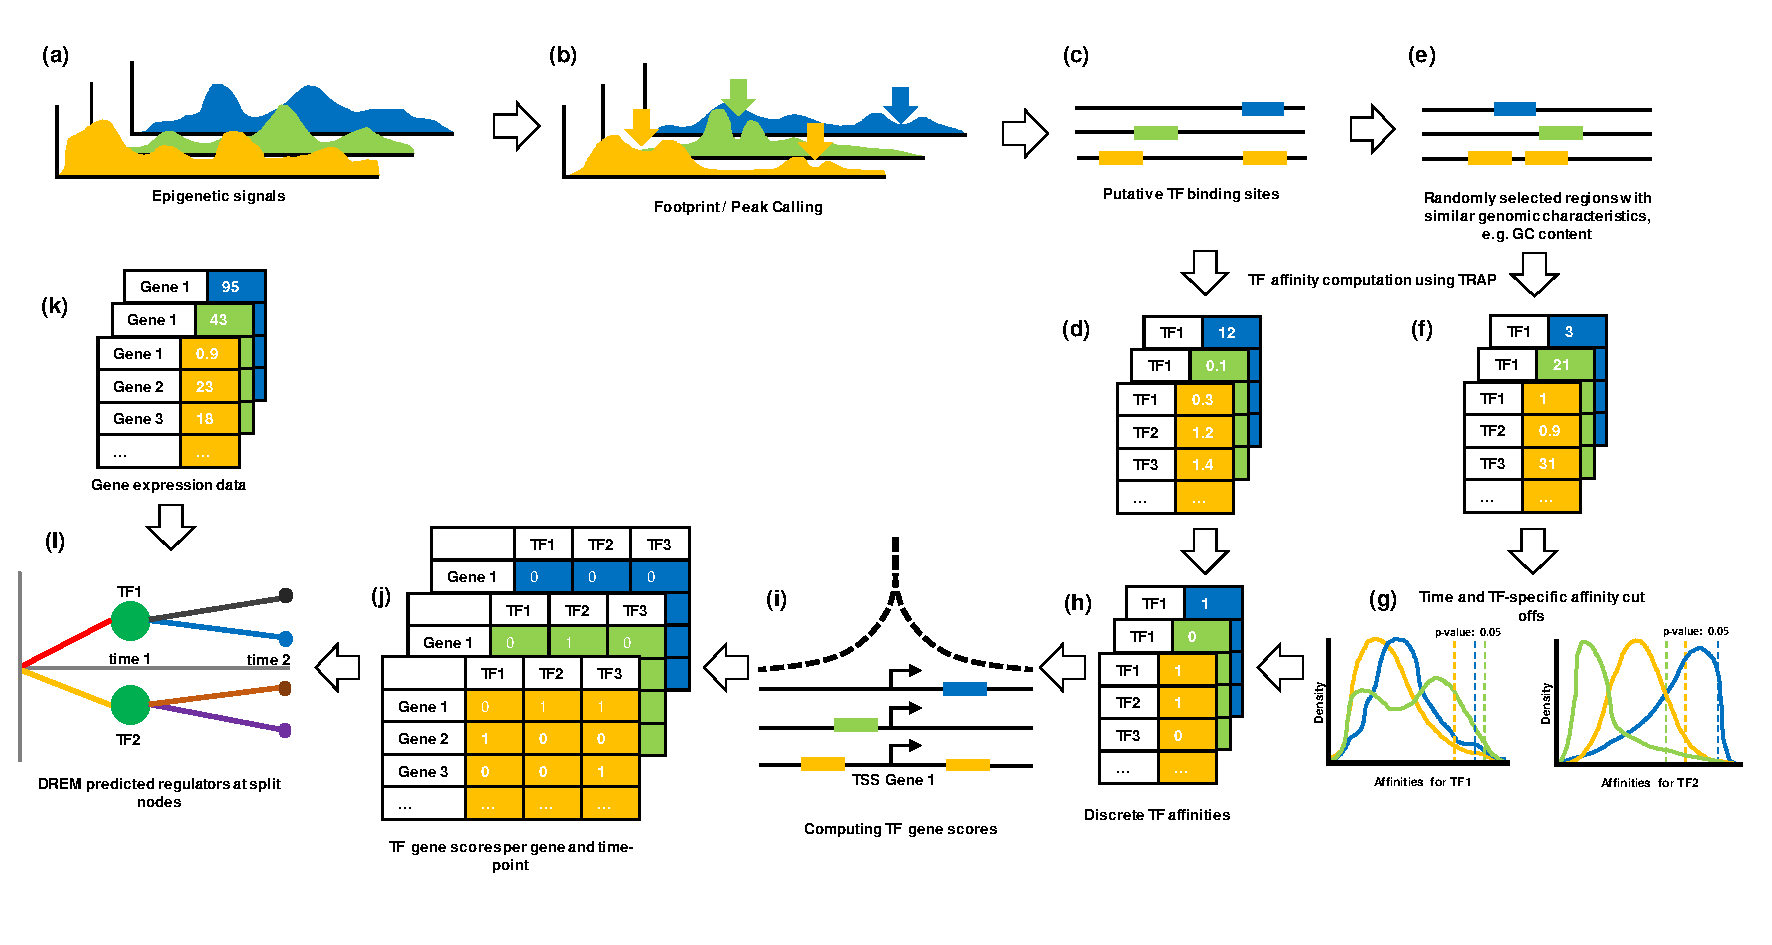
\includegraphics[width=\textwidth]{epicdrem.pdf}
\end{center}
\caption{Overview on the EPIC-DREM approach: Note that in this Figure, different time points are indicated by different colours. First, epigenetic data, e.g. DNase1 experiments, are conducted for different points (a).
Next, putative TF binding sites are identified by peak and/or footprint calling (b,c) and annotated with TF affinities (d). 
From the putative binding sites, a random set of genomic regions is chosen (e) and annotated with TF affinities as well (f). By applying a p-value cut-off on the distribution of TF affinities calculated on the random regions (g),
a suitable, TF specific affinitiy threshold is choosen to discretise the original TF affinities (h). Using the default TEPIC TF-gene score formulation (i), a TF-gene interaction matrix (j) is computed. Together with gene expression data (k),
the sparse matrix (j) can be used as input for DREM (l) to identify potential key regulators of expression changes in time series data.}
\label{epicdrem}
\end{figure}

\subsubsection*{Thresholded TF affinities}
In some applications it is required to make a binary decision whether a factor is binding or not. 
To infer this information from TF affinities, \textit{TEPIC} allows the computation of a TF specific affinity threshold by calculating TF affinities on a randomly selected set of genomic regions. When selected by TEPIC, these regions show similar characteristics compared to the provided regions (GC content and length). 
Alternatively a set of background regions can be provided by the user.
By applying a user defined p-value on the distribution of affinities computed on the random regions, a threshold is chosen. 
Per TF, all affinities that are smaller than the selected threshold, are set to zero, thus a sparse matrix with TF-gene interactions can be generated. 

\subsubsection*{Required input}
In addition to the input mentioned above, a reference genome in 2bit format is required. 
Optionally, the user can provide a bed file containing background regions. 
These replace the automated generation of background sequences. 

\subsubsection*{Output}
The following output files are generated in addition:
\begin{enumerate}
\item TF affinities for all selected \textit{PSEMs} in the regions provided by the user that passed the filtering step, where all affinities below the TF specific thresholds are set to 0.
\item (Length normalised) TF gene scores for all selected \textit{PSEMs} calculated as described above (optionally including peak features) using the thresholded affinities.
\item A sparse representation of TF gene interactions.
\end{enumerate}

Either (2) or (3) can be combined with RNA-seq data and used as input for \textit{DREM}.

\bibliographystyle{plain}
\bibliography{Description}
\end{document} 
